\documentclass{article}
    \usepackage{xparse}
    \usepackage[margin=2cm]{geometry}
	\usepackage{enumerate} 
    \usepackage{textcomp}
	\frenchspacing
	\linespread{1.2}

    \usepackage[polish]{babel}
    \usepackage[utf8]{inputenc}
    \usepackage{polski}

	\usepackage{amsthm}
	\usepackage{amsmath}
	\usepackage{amsfonts}
	\usepackage{float}
    \usepackage{diagbox}
	\usepackage{hhline}
	\usepackage{graphicx}
	\usepackage{multirow}
	\usepackage{mathtools}
	\usepackage{hyperref}


	\theoremstyle{definition}
	\newtheorem{zadanie}{Zadanie}[subsection]
	\renewcommand{\thezadanie}{\arabic{zadanie}}

\title{\textbf{Query-by-Sketch: Scaling Shortest Path Graph Queries on Very Large Networks}}

\author{Paweł Polerowicz}
\date{Styczeń 2024}

\begin{document}
    \maketitle
    \section{Wiadomości wstępne}
    
    \subsection{Informacje o artykule}
    \begin{itemize}
        \item Tytuł: Query-by-Sketch: Scaling Shortest Path Graph Queries on Very Large Networks
        \item Autorzy: Ye Wang, Qing Wang, Henning Koehler, Yu Lin
        \item Data publikacji: 2021
        \item miejsce publikacji: Proceedings of the 2021 International Conference on Management of Data
    \end{itemize}
    
    \subsection{Słowniczek pojęć}

    \begin{tabular}{|l | l | } 
        \hline
        Oznaczenie & Znaczenie \\
        \hline\hline
        $G(V,E)$ & graf (tu nieskierowany i spójny) \\ 
        \hline
        $P_{uv}$ & zbiór najkrótszych ścieżek między wierzchołkami $u$ i $v$ \\ 
        \hline
        $d_G(u, v)$ & długość najkrótszej ścieżki między $u$ i $v$ \\ 
        \hline
        $R \subset V$ & zbiór punktów orientacyjnych (ang. \textit{Landmarks}) \\ 
        \hline
        $L(v) = \{(r_1, \delta_{vr_1}),\cdots,(r_n, \delta_{vr_n})\}$ & zbiór etykiet wierzchołka $v$ \\ 
        \hline
        $\delta_{vr_i}$ & $= d_G(v, r_i)$ \\ 
        \hline
        $L = \{L(v)\}_{v \in V}$ & etykietowanie nad $G$\\ 
        \hline
        $size(L) = \sum_{v \in V}|L(v)|$ & rozmiar etykietowania \\ 
        \hline
    \end{tabular}\\
    
    \subsection{Plan prezentacji}
        W ramach niniejszej prezentacji zreferujemy artykuł \textit{Query-by-Sketch: Scaling Shortest Path Graph Queries on Very Large Networks}, przedstawiający metodę QbS. Składa się ona z trzech algorytmów. Pierwszy z nich służy jako przetwarzanie wstępne i są wykonywany raz i wyznacza etykietowanie $L$ dla grafu $G$. Drugi tworzy szkic danych dla pary wierzchołków $u$ i $v$ na podstawie etykietowania $L$. Ostatni wyznacza dokładną odpowiedź, wykorzystując przeszukiwanie kierowane szkicem. Złożoności algorytmów to kolejno $O(|R||E|)$, $O(|R|^4)$ (z możliwością ograniczenia do $O(|R|^2)$) oraz $O(|E| + |R||V|)$, gdzie R jest zbiorem punktów orientacyjnych.

    \subsection{Motywacja}
        Podczas poprzednich prezentacji omawialiśmy struktury wykorzystujące szkice danych do efektywnego pamięciowo przechowywania informacji o strumieniowanym grafie. W szczególności rozważaliśmy takie konstrukcje, które pozwalały na uzyskiwanie szybkich odpowiedzi na zapytania o istnienie i wagę krawędzi między dwoma wierzchołkami, a także łączną wagę krawędzi wchodzących i wychodzących z danego wierzchołka. Niemniej jednak często zależy nam na wykonywaniu bardziej skomplikowanych operacji. Jedną z typowych może być wyznaczanie najkrótszych ścieżek między wierzchołkami. Rozwiązania tego problemu mogą znaleźć swoje zastosowanie np. w nawigacji GPS lub w analizie sieci społecznościowych. W obu przypadkach mamy do czynienia z grafami o nierzadko ogromnych rozmiarach. Sprawia to, że klasyczne i dobrze przebadane algorytmy mogą okazać się nieskuteczne, ze względu na konieczność przeglądu zatrważającej liczby krawędzi lub wykorzystywania dodatkowej pamięci o niepraktycznym rozmiarze. Dodatkowo niejednokrotnie możemy być zainteresowani wyborem nie jednej ścieżki, lecz pewnego zbioru najkrótszych lub prawie najkrótszych ścieżek. Śledząc wysiłki autorów artykułu, spróbujemy znaleźć metodę wyznaczania grafu najkrótszych ścieżek w sposób wydajny czasowo i przy użyciu rozsądnej ilości pamięci. 
    
    \section{Problem}
    
    \subsection{Sformułowanie problemu}

        \subsubsection*{2-hop distance cover (dwu-przeskokowe pokrycie odległości :))}
            Etykietowanie $L$ grafu $G$ stanowi 2-hop distance cover, jeśli zachodzi 
            \[
                \forall_{u,v \in V} d_G(u, v) = min\{\delta_{ur} + \delta_{vr} : (r, \delta_{ur}) \in L(u), \delta_{vr} \in L(v)\}    
            \]
            Innymi słowy, wymagamy, aby dla każdej pary wierzchołków, ich etykiety zawierały co najmniej jeden wspólny punkt orientacyjny leżący na jednej z najkrótszych ścieżek je łączących. 
    
        \subsubsection*{SPG (graf najkrótszych ścieżek)}
            Dla dowolnych dwóch wierzchołków $u$ i $v$, graf najkrótszych ścieżek (SPG) między $u$ i $v$ to podgraf $G_{uv}$ grafu, gdzie:
            \begin{enumerate}
                \item $V(G_{uv}) = \bigcup_{p \in P_{uv}} V(p)$
                \item $E(G_{uv}) = \bigcup_{p \in P_{uv}} E(p)$
            \end{enumerate}
            Graf ten nie jest więc po prostu podgrafem indukowanym przez $\bigcup_{p \in P_{uv}} V(p)$, gdzie $P_{uv}$ to zbiór najkrótszych ścieżek między wierzchołkami $u$ i $v$. Każda jego krawędź musi być bowiem częścią najkrótszej ścieżki między $u$ i $v$. 

        \subsubsection*{Problem SPG}
            Niech $G = (V, E)$ oraz $u,v \in V$. Problem SPG polega na znalezieniu odpowiedzi na zapytanie $SPG(u,v)$, czyli grafu najkrótszych ścieżek $G_{uv}$ dla $G$. W niniejszej prezentacji będziemy dla uproszczenia zakładali, że graf jest nieskierowany, spójny i nie jest ważony. W ogólności jednak te ograniczenia są możliwe do zrelaksowania. 

    \subsection{Główne idee rozwiązań}

    \section{Przegląd poprzednich rozwiązań}
        
    \subsection{Klasyczne algorytmy}

        \subsection{Algorytmy dokładne dla dużych grafów}

        \subsection{Algorytmy aproksymacyjne}

            
    \section{QbS}
    
    \subsection{Idea}

    \begin{figure}[!tbh]
        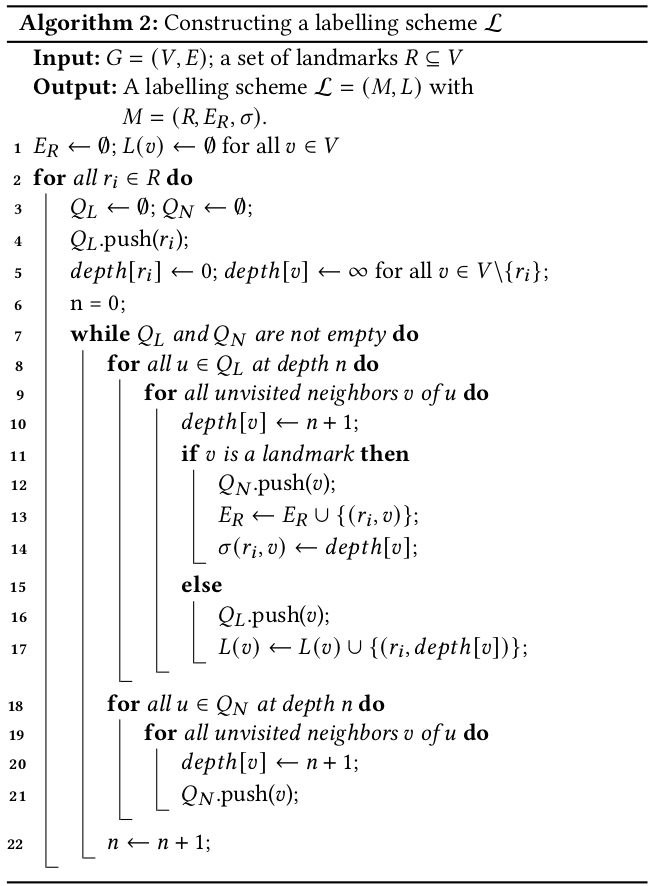
\includegraphics[width=11cm]{img/algorithm_2.png}
        \centering
        \label{fig:alg2}
        \caption{Pseudokod procedury etykietowania}
    \end{figure}


    \begin{figure}[!tbh]
        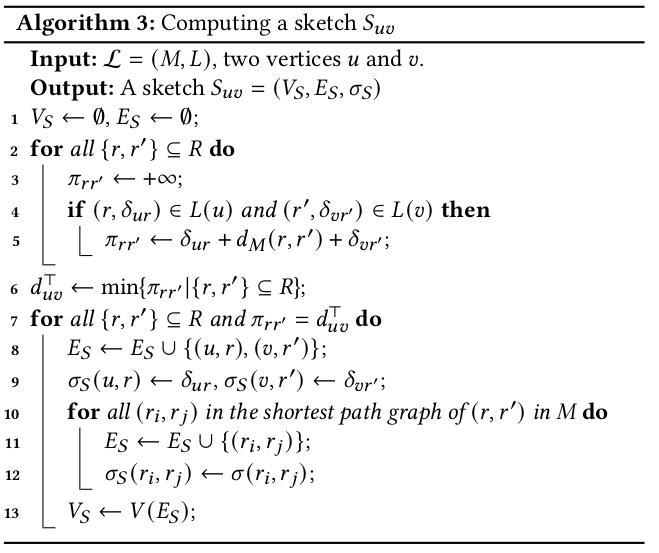
\includegraphics[width=11cm]{img/algorithm_3.png}
        \centering
        \label{fig:alg3}
        \caption{Pseudokod procedury szkicowania}
    \end{figure}


    \begin{figure}[!tbh]
        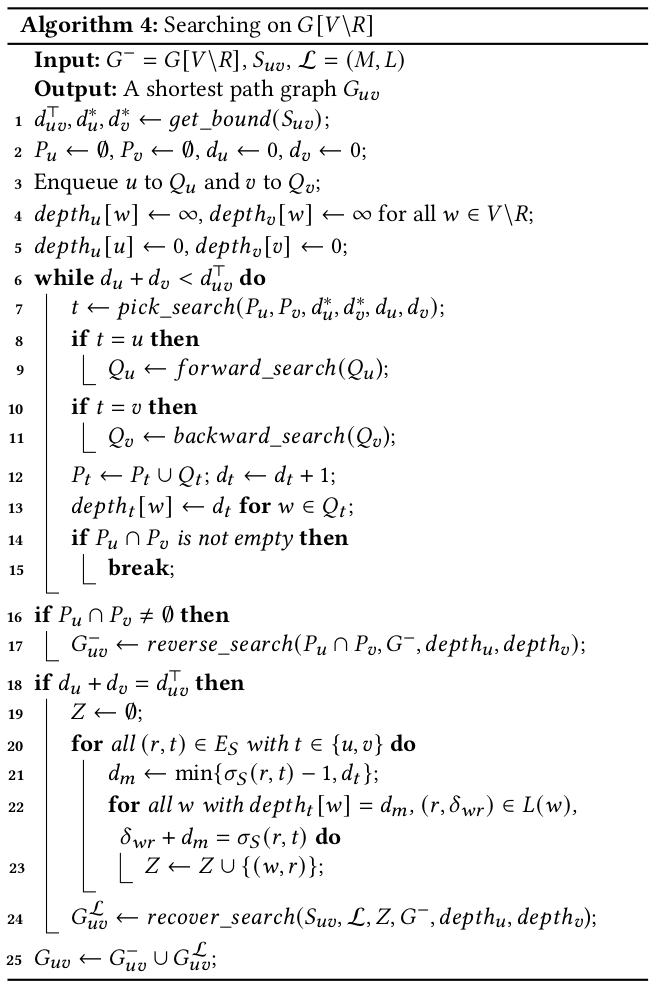
\includegraphics[width=11cm]{img/algorithm_4.png}
        \centering
        \label{fig:alg4}
        \caption{Pseudokod przeszukiwania kierowanego szkicem}
    \end{figure}

    \subsection{Przykład}
     
    \subsection{Etykietowanie}
        Niech $G = (v, E)$ - graf, $R \subset V$ - zbiór punktów orientacyjnych spełniający $|R| \ll |V|$. Schemat QbS zaczyna się od przetwarzania wstępnego, którego celem jest znalezienie kompaktowej reprezentacji najkrótszych ścieżek pomiędzy punktami orientacyjnymi, zwanej meta-grafem grafu $G$. Następnie, bazując na tymże meta-grafie, tworzymy etykietowanie, każdemu wierzchołkowi przypisując każdemu wierzchołkowi taką etykietę, aby móc efektywnie policzyć szkic dla zapytania $SPG(u, v)$  dla dowolnych $u$ i $v$.

        \subsubsection*{Meta-graf}
            Meta grafem nazywamy trójkę $M = (R, E_R, \sigma)$, gdzie $E_R \subset R \times R$ jest zbiorem krawędzi postaci $(r, r')$ spełniających warunek, że przynajmniej jedna najkrótsza ścieżka między $r$ i $r'$ w oryginalnym nie przechodzi przez żaden inny punkt orientacyjny. $\sigma: E_R \rightarrow \mathbb{N}$ przypisuje każdej krawędzi w $E_R$ wagę równą długości najkrótszej ścieżki. 

        \subsubsection*{System etykietowania (ang. \textit{Labelling scheme})}
            System etykietowania $\mathcal{L} = (M,L)$ składa się z meta-grafu M oraz etykietowania, które przypisuje każdemu wierzchołkowi $u \in V \setminus R$ etykietę $L(u)$ taką że:
            \[ 
                L(u) = \{(r, \delta_{ur}) : r \in R, \delta_{ur} = d_G(u,r), (\exists p \in P_{ur})(V(p) \cap R {r}) \}
            \]
            Innymi słowy, para $(r, \delta_{ur})$ jest częścią etykiety $L(u)$ tylko, jeśli istnieje co najmniej jedna najkrótsza ścieżka między $u$ i $r$, która nie zawiera innych punktów orientacyjnych. 

            Algorytm etykietowana ukazano na obrazku \hyperref[fig:alg2]{1}. Wykonujemy BFS dla każdego punktu orientacyjnego $r$. Wykorzystujemy dwie kolejki do przechowywania odwiedzonych wierzchołków, zależnie od tego, czy mają one zostać zaetykietowane z wykorzystaniem $r$, czy też nie. Wszystkie wierzchołki oprócz $r$ są na początku niezaetykietowane. Dla każdego wierzchołka w kolejce zaetykietowanych z $r$ na n-tym poziomie BFS rozpatrujemy nieodwiedzonych sąsiadów i oznaczamy ich jako odwiedzonych. Jeśli dany sąsiad jest punktem orientacyjnym to dodajemy krawędź do meta-grafu i ustawiamy głębokość jako dystans w funkcji $\sigma$. W przeciwnym przypadku dodajemy parę $(r, depth(v))$ do etykiety $L(V)$, a sam wierzchołek $v$ do kolejki wierzchołków zaetykietowanych z $r$. Następnie rozpatrujemy kolejkę niezaetykietowanych na n-tym poziomie i wszystkich nieodwiedzonych sąsiadów dodajemy do kolejki niezaetykietowanych. Powtarzamy na kolejnych poziomach aż do przetworzenia wszystkich wierzchołków. Przykład ukazano na rysunku \hyperref[fig:label]{4}

            \begin{figure}[!tbh]
                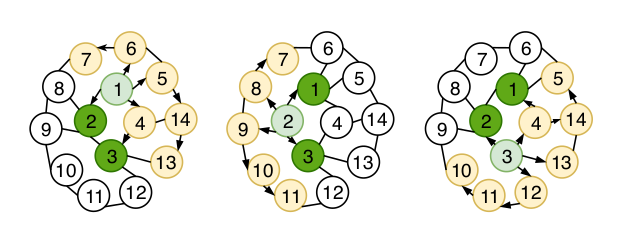
\includegraphics[width=11cm]{img/labelling.png}
                \centering
                \label{fig:label}
                \caption{Przykład etykietowania kolejno dla wierzchołków 1, 2 i 3}
            \end{figure}

    \subsection{Szkicowanie grafu najkrótszych ścieżek}
        Aby móc efektywnie odpowiedzieć na zapytanie $SPG(u,v)$ niezbędne jest przygotowanie szkicu danych dla wierzchołków $u$ i $v$. Będzie on oparty o schemat $\mathcal{L}$.
        
        \subsubsection*{Szkic}
            Szkicem dla $SPG(u,v)$ na podstawie $\mathcal{L}$ nazywamy trójkę $S_{uv} = (V_S, E_S, \sigma_S)$, gdzie $V_S = \{u,v\} \cup R$ jest zbiorem wierzchołków, $E_S$ zbiorem krawędzi, a $\sigma_S \rightarrow \mathbb{N}$ zachowuje $\sigma_S(u', v') = d_G(u', v')$. Trójka ta zachowuje warunek, że $E_S$ zawiera jedynie krawędzie na ścieżkach między $u$ i $v$ o minimalnej długości, a więc:
            \[
                d_{uv}^T = min_{(r,r')}\{\delta_{ru} + d_M(r,r') + \delta_{r'v} : (r,\delta_{ru}) \in L(u), (r',\delta_{r'v}) \in L(v)\}
            \]
            Oczywiście, zachodzi własność $d_{uv}^T \geq d_G(u,v)$. Algorytm ukazany na rysunku \hyperref[fig:alg3]{3} tworzy omawiany szkic. Najpierw, zbiory wierzchołków i krawędzi w szkicu są puste. Zaczynamy od sprawdzenia wszystkich par punktów orientacyjnych, wyznaczając najkrótszą ścieżkę z $u$ do $v$ przechodzącą przez oba te punkty używając etykiet i meta-grafu. Najkrótsza otrzymana ścieżka to $d_{uv}^T$. Następnie, dla wszystkich wyznaczonych ścieżek o takiej długości, dodajemy ich krawędzie do zbioru krawędzi szkicu, łącznie z krawędziami łączącymi $u$ i $v$ z punktami obserwacyjnymi. Analogicznie, do zbioru dodajemy wszystkie wierzchołki na tych ścieżkach.
    
    \subsection{Przeszukiwanie kierowane}
        
    \subsection{Poprawność}

    \subsection{Złożoność pamięciowa}
    
    \subsection{Złożoność czasowa (szkic)}

    \subsection{Urównoleglenie}
        Łatwo pokazać, że dla danego zbioru punktów orientacyjnych $R$ w $G$, istnieje dokładnie jeden system etykietowania $\mathcal{L}$ spełniający definicję, jego wybór jest więc oczywiście deterministyczny. Pozwala to łatwe urównoleglenie algorytmu etykietowania.

    \subsection{Zależność od liczby punktów orientacyjnych}
    
    \section{Zakończenie}
    Dziękuję słuchaczom za uwagę i życzę miłego dnia. 
    
\end{document}